%%%% PROCESAR con PdfLaTeX !!!!!


\documentclass[12pt]{book}
\usepackage{geometry}\geometry{top=2cm,bottom=2cm,left=3cm,right=3cm}
\usepackage{amssymb}
\usepackage{amsmath}
\usepackage{graphicx}
\usepackage{txfonts}




\begin{document}
\thispagestyle{empty}

\begin {center}

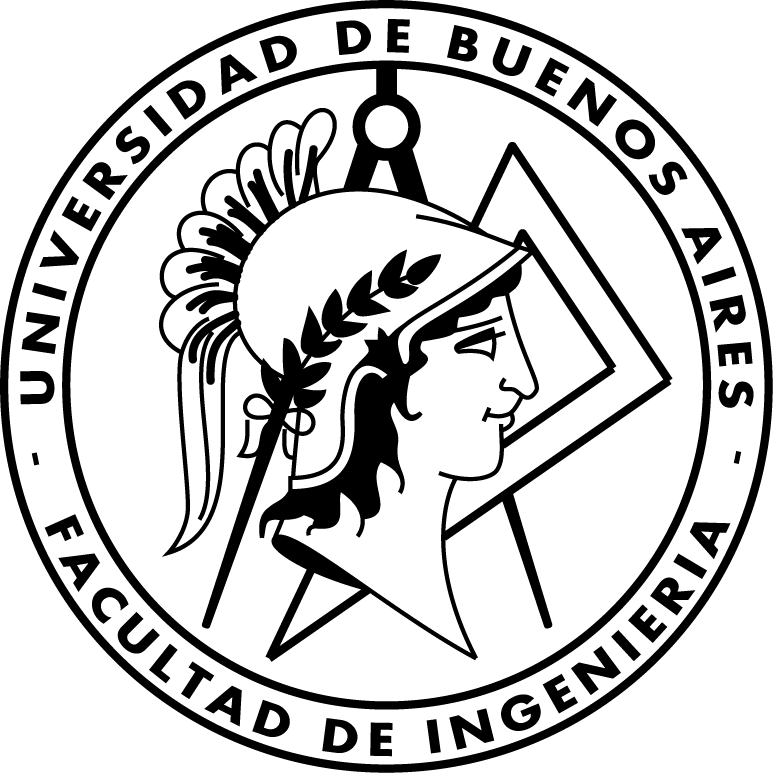
\includegraphics[scale=.4]{Logo-fiuba_big.png}

\medskip
UNIVERSIDAD DE BUENOS AIRES

Facultad de Ingenier\'ia

Departamento de Economia, Organizaci\'on y legal


\vspace{3cm}


\textbf{\large 7114 Modelos y Optimizaci\'on 1}

\vspace{2cm}


Este es un modesto aporte para los alumnos de la f\'acultad de ingenier\'ia  de la UBA de las carreras de sistemas e inform\'atica.
De ninguna man\'era pretende ser una guia de estudio, ni remplaza las clases presenciales, el material oficial de la catedra esta disponible en el web site de la m\'ateria.
\\
wwww.ModelosUno.com.ar

\end {center}


\vspace{2.5cm}

\noindent Autor: Isaac Edgar Camacho Ocampo
 
\noindent Carrera: Licenciatura en An\'alisis de sistemas

\vspace{1cm}

\vspace{1cm}

\noindent Buenos Aires, 2019

\newpage



\textbf{CONCEPTOS PREVIOS}
\begin{enumerate}
	\item \textbf{Eficiencia:} Producir mas con menos recursos o productividad.
	\item \textbf{Eficacia:} Lograr el resultado aunque se consuman muchos recursos.
	\item \textbf{Costo de oportunidad:} Es el costo de producir una unidad de un bien.
	\item \textbf{Contribucion marginal:} Ganancia neta.
\end{enumerate}
\title{\textbf{TRABAJANDO CON MODELOS MATEMATICOS LINEALES}}
\textbf{¿Que es modelizar?} Es hacer una simplificacion de la realidad y nosotros trabajamos con esa simplificacion ya que la realidad es muy compleja.
\\
\textbf{¿Para que hacer un modelo?}
\begin{itemize}
\item \textbf{Economia de recursos:} Al igual que en la ingenieria civil cuando se hacen planos para representar una obra (ya que no seria l\'ogico hacer el edificio y ante un error rehacerlo), cuando modelamos un problema usando programacion lineal y dada la escazes de recursos, es mas eficiente trabajar sobre modelos.
\item \textbf{Eficiencia}: de nuevo so no tengo recursos limitantes entonces trabajo sobre la realidad y no modelo nada.
\item \textbf{simplicidad}: puedo mediante abstracci\'on lograr un modelo mas sencillo y eliminar la complejidad inherente del problema.
\item \textbf{En resumen es mejor que hacer multiples ensayos.}
\end{itemize}
Los mod\'elos se aplican a problemas de desici\'on y este existe cuando existen formas alternativas de actuar, con distintos resultados y diferentes eficiencias para lograr el objetivo es decir existen dudas respecto del curso alternativo a utilizar.
\\
\\
\textbf{Elementos de un modelo}
\\
\\
\textbf{Hipótesis y supuestos:} Para simplificar el modelo se delimita el sistema en estudio a través de las hipótesis y
supuestos simplificativos. Así se comienza a transformar el sistema físico en un modelo simbólico.
Las hipótesis deben ser probadas científicamente. Los supuestos son hipótesis que no pueden probarse.
\\
\textbf{Ejemplos:}
Si estamos modelando una panaderia, y el recurso agua no es limitante y por otro no se dice nada de 				la venta de lo producido podemos agregar las hipotesis
\begin{enumerate}
	\item 	
	\textit{Hay agua suficiente para todos los procesos}
	\item
	\textit{Se vende todo lo que se produce}
\end{enumerate}
\textbf{Objetivo: }Mide la eficiencia de nuestro sistema y lo que buscamos es hallar la merjo solucion. El objetivo surge como respuesta a tres preguntas:
\\¿Qué hacer? es decir que es lo que queremos determinar.
\\¿Cuándo? (período de tiempo) puede ser un mes o año o un periodo t si no se especifica.
\\¿Para qué? para maximizar ganancias, o minimizar costos, nunca ambos a la vez.
\\
\\
\textbf{Actividad}
Proceso unitario que se realiza en el sistema físico caracterizado por consumir recursos
y/o generar un resultado económico y/o indicar un estado, por ejemplo producir un bien o indicar si se finaliz\'o un proceso.
\\
\\
\textbf{Variables}
Son las que miden o indican el estado de una actividad.
Las que miden pueden ser continuas o enteras.
Las que indican son, generalmente, variables (0,1) o bivalentes

\end{document}
